\chapter{Malla curricular \YYYY}\label{chap:GeneralInfo}

\section{Clasificaci�n de los cursos por niveles}
De acuerdo a la \textit{Computing Curricula}, los cursos son clasificados en 3 niveles: Introductorios, Intermedios y Avanzados
como puede ser observado en la Figura~\ref{fig:niveles}. Los abordajes posibles para iniciar una carrera de este tipo de 
acuerdo al est�ndar son: Imperativo, Objetos, Funcional, Visi�n amplia, Algoritmos, Hardware.

Los cursos de nivel intermedio pueden tener las siguientes orientaciones: Basado en t�picos, comprimido, 
basado en sistemas, orientado a la internet. Los cursos de tercer nivel tienen por objetivo abrir 
varias posibilidades de especializaci�n por lo que no est�n divididos en categor�as.

\begin{figure}[ht]
   \centering
   \includegraphics[width=13cm]{\OutputFigDir/course-levels}
   \caption{Orientaciones de los cursos por niveles.}
   \label{fig:niveles}
\end{figure}

Esta propuesta de malla curricular est� basada en el abordaje funcional en el nivel introductorio y orientado 
a internet en el nivel intermedio. El abordaje funcional fue escogido porque nos da la oportunidad de 
concentrarnos en el desarrollo algoritmico del alumno y no en el aprendizaje de sintaxis de un lenguaje 
en particular. El abordaje orientado a la web se escogi� porque hacia eso apuntan las tendencias 
futuras de la computaci�n.

\section{Codificaci�n de los cursos}
Los cursos se encuentran codificados bajo el esquema que se muestra en la Figura~\ref{fig:course-number}:

\begin{figure}[ht]
   \centering
   \includegraphics[width=13cm]{\OutputFigDir/course-number}
   \caption{Esquema de codificaci�n para los cursos.}
   \label{fig:course-number}
\end{figure}

El �rea de un curso esta determinada por sus 2 primeras letras. Los posibles c�digos para estas l�neas son:
\input{\OutputTexDir/areas-description}

\begin{landscape}
\section{Malla curricular por semestres}\label{sec:courses-by-semester}
La relaci�n de cursos se muestra a continuaci�n:
\input{\OutputTexDir/tables-by-semester}

\OnlySPC{Es importante resaltar que todos los semestres podr�an ser completados con cursos extras de acuerdo al perfil de la instituci�n.}
\end{landscape}

\section{Estad�sticas de la malla curricular}
Esta propuesta puede ser analizada por el n�mero de cr�ditos dedicados a cada �rea
%horas de clase de las mismas
y por niveles de cursos (Introductorios, Intermedios, Avanzados y Proyectos).
\vspace{0.5cm}

\begin{figure}[h!]
      \centering
      \includegraphics[width=10cm]{\OutputFigDir/pie-credits}
      \label{fig:pie-credits}
      \caption{Distribuci�n de cursos por �reas considerando creditaje.}
\end{figure}

\input{\OutputTexDir/distribution-area-by-semester}

\begin{figure}[h!]
      \centering
      \includegraphics[width=10cm]{\OutputFigDir/pie-by-levels}
      \label{fig:pie-niveles}
      \caption{Distribuci�n de cr�ditos por niveles de cursos.}
\end{figure}

\begin{landscape}
\section{Visi�n gr�fica de la Malla curricular}\label{sec:vision-grafica}
\vspace{-0.3cm}Este documento tambi�n puede ser analizado desde el punto de vista de los prerequisitos de forma gr�fica.
\begin{figure}[h!]
      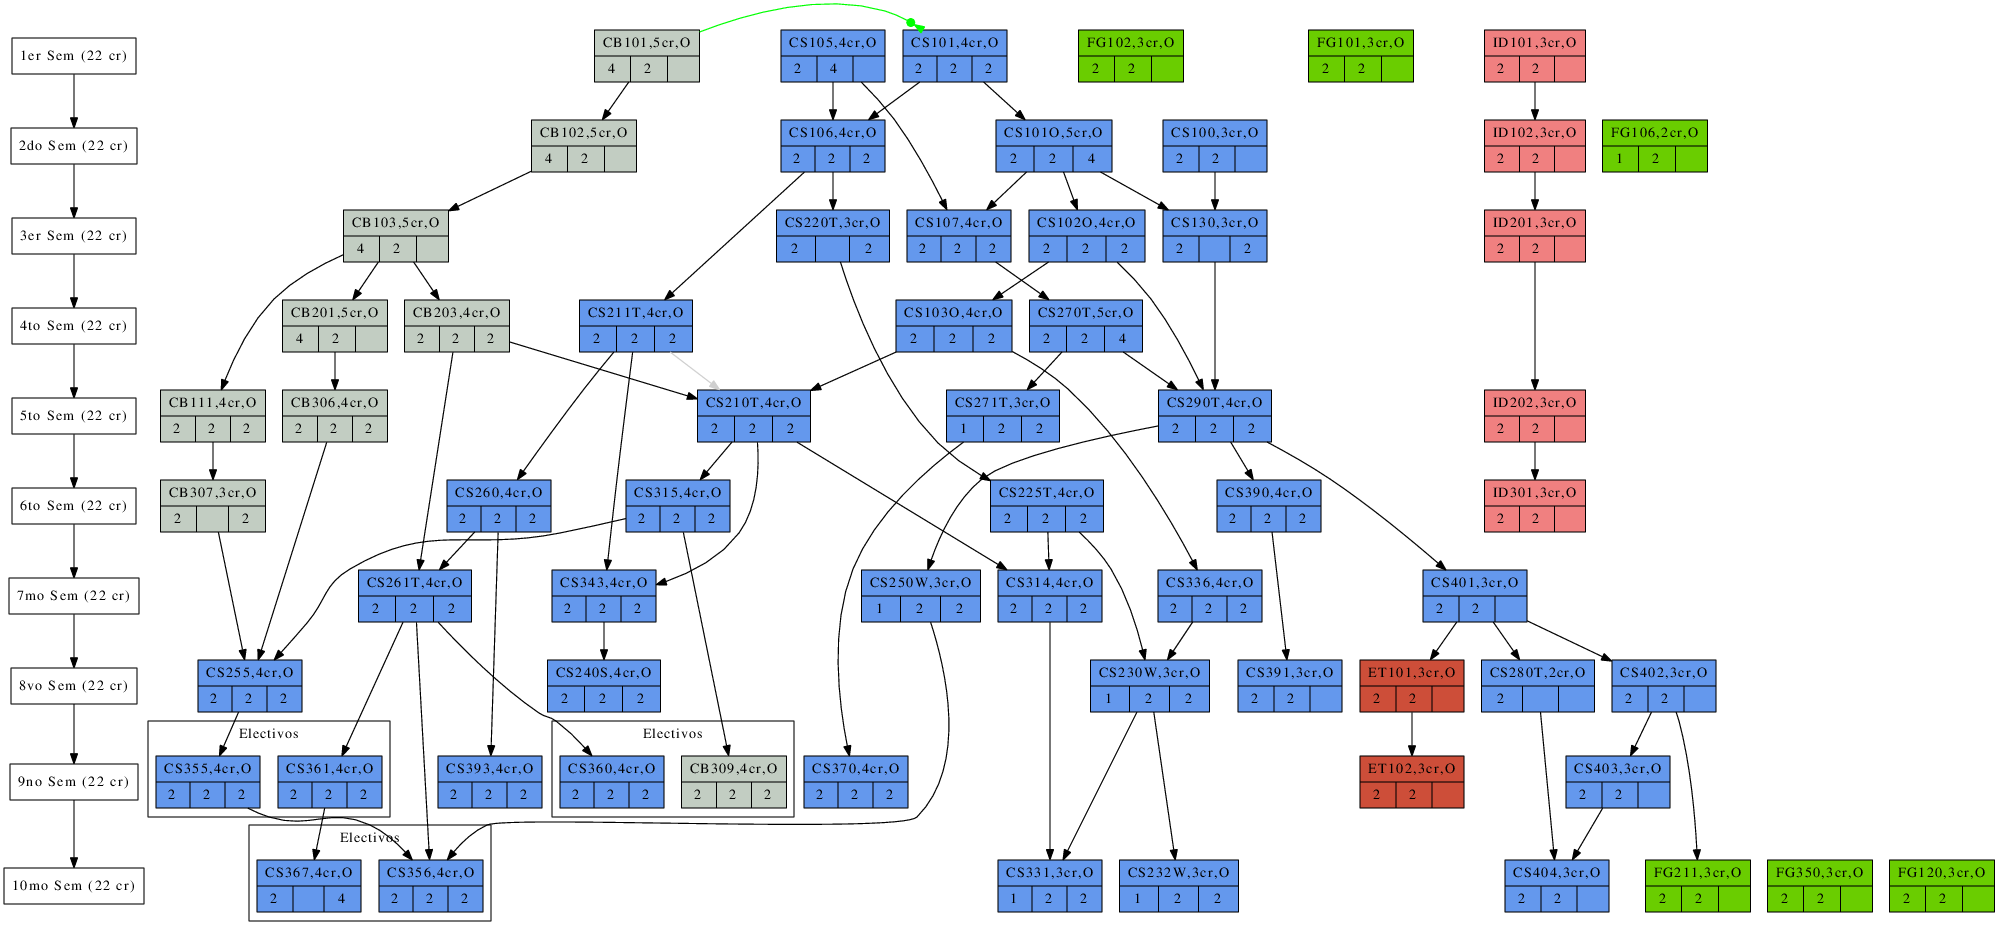
\includegraphics[width=23cm]{\OutputFigDir/small-graph-curricula.ps}
      \label{fig:malla-curricular}
      \caption{Malla curricular \SchoolFullName}
\end{figure}
\end{landscape}

\section{Compatibilidad de la carrera con relaci�n a estandares internacionales}
En esta secci�n presentamos la distribuci�n de cursos por �reas de concentraci�n en 
contraste con las propuestas internacionales de las carreras de la \textit{Computing Curricula} 
de IEEE-CS/ACM.

Es necesario notar que \underline{en algunos casos las materias podr�an aparecen en m�s de un eje} 
pues tienen contenido de m�s de una �rea. 
Por ejemplo, la materia de sistemas operativos contiene unidades de aplicaci�n 
que pueden ser clasificadas en Tecnolog�a de Informaci�n pero al mismo tiempo contiene fundamentos 
de como est� estructurado un Sistema Operativo que es del eje de Ciencia de la Computaci�n. 
En estos casos el creditaje ha sido divido entre los ejes correspondientes.
\input{\OutputTexDir/list-of-courses-per-area}

Considerando esta distribuci�n, las figuras \ref{fig:comparing-curves-\currentarea-\currentinstitution-with-CE} 
a la \ref{fig:comparing-curves-\currentarea-\currentinstitution-with-SE} 
nos permiten tener una visi�n gr�fica de esta malla curricular frente a las propuestas de 
carreras presentadas por IEEE-CS/ACM en la \textit{Computing Curricula}
\input{\OutputTexDir/comparing-with-standards}

\begin{landscape}
\section{Distribuci�n de t�picos por curso}\label{sec:topics-by-course}
Las siguientes tablas nos muestran la distribuci�n de todos los t�picos del 
cuerpo del conocimiento de \ac{\currentarea} en todos los cursos.
\section{Distribuci�n de t�picos por curso}\label{sec:topics-by-course}
Las siguientes tablas nos muestran la distribuci�n de todos los t�picos del 
cuerpo del conocimiento de \ac{\currentarea} en todos los cursos.
\section{Distribuci�n de t�picos por curso}\label{sec:topics-by-course}
Las siguientes tablas nos muestran la distribuci�n de todos los t�picos del 
cuerpo del conocimiento de \ac{\currentarea} en todos los cursos.
\input{\OutputTexDir/topics-by-course}
\end{landscape}

\begin{landscape}
\section{Resultados esperados distribu�dos por curso}\label{sec:outcomes-by-course}
Las siquientes tablas nos muestras una visi�n global de los resultados que se esperan lograr en cada 
curso de la presente malla curricular. 
La lista completa de resultados esperados se encuentra en la Secci�n:~\ref{sec:outcomes}.
\section{Resultados esperados distribu�dos por curso}\label{sec:outcomes-by-course}
Las siquientes tablas nos muestras una visi�n global de los resultados que se esperan lograr en cada 
curso de la presente malla curricular. 
La lista completa de resultados esperados se encuentra en la Secci�n:~\ref{sec:outcomes}.
\section{Resultados esperados distribu�dos por curso}\label{sec:outcomes-by-course}
Las siquientes tablas nos muestras una visi�n global de los resultados que se esperan lograr en cada 
curso de la presente malla curricular. 
La lista completa de resultados esperados se encuentra en la Secci�n:~\ref{sec:outcomes}.
\input{\OutputTexDir/outcomes-by-course}
\end{landscape}
